\appendix
        \begin{frame}
        \frametitle{Candoia Data Schema}
                \begin{figure}
                    \centering
                    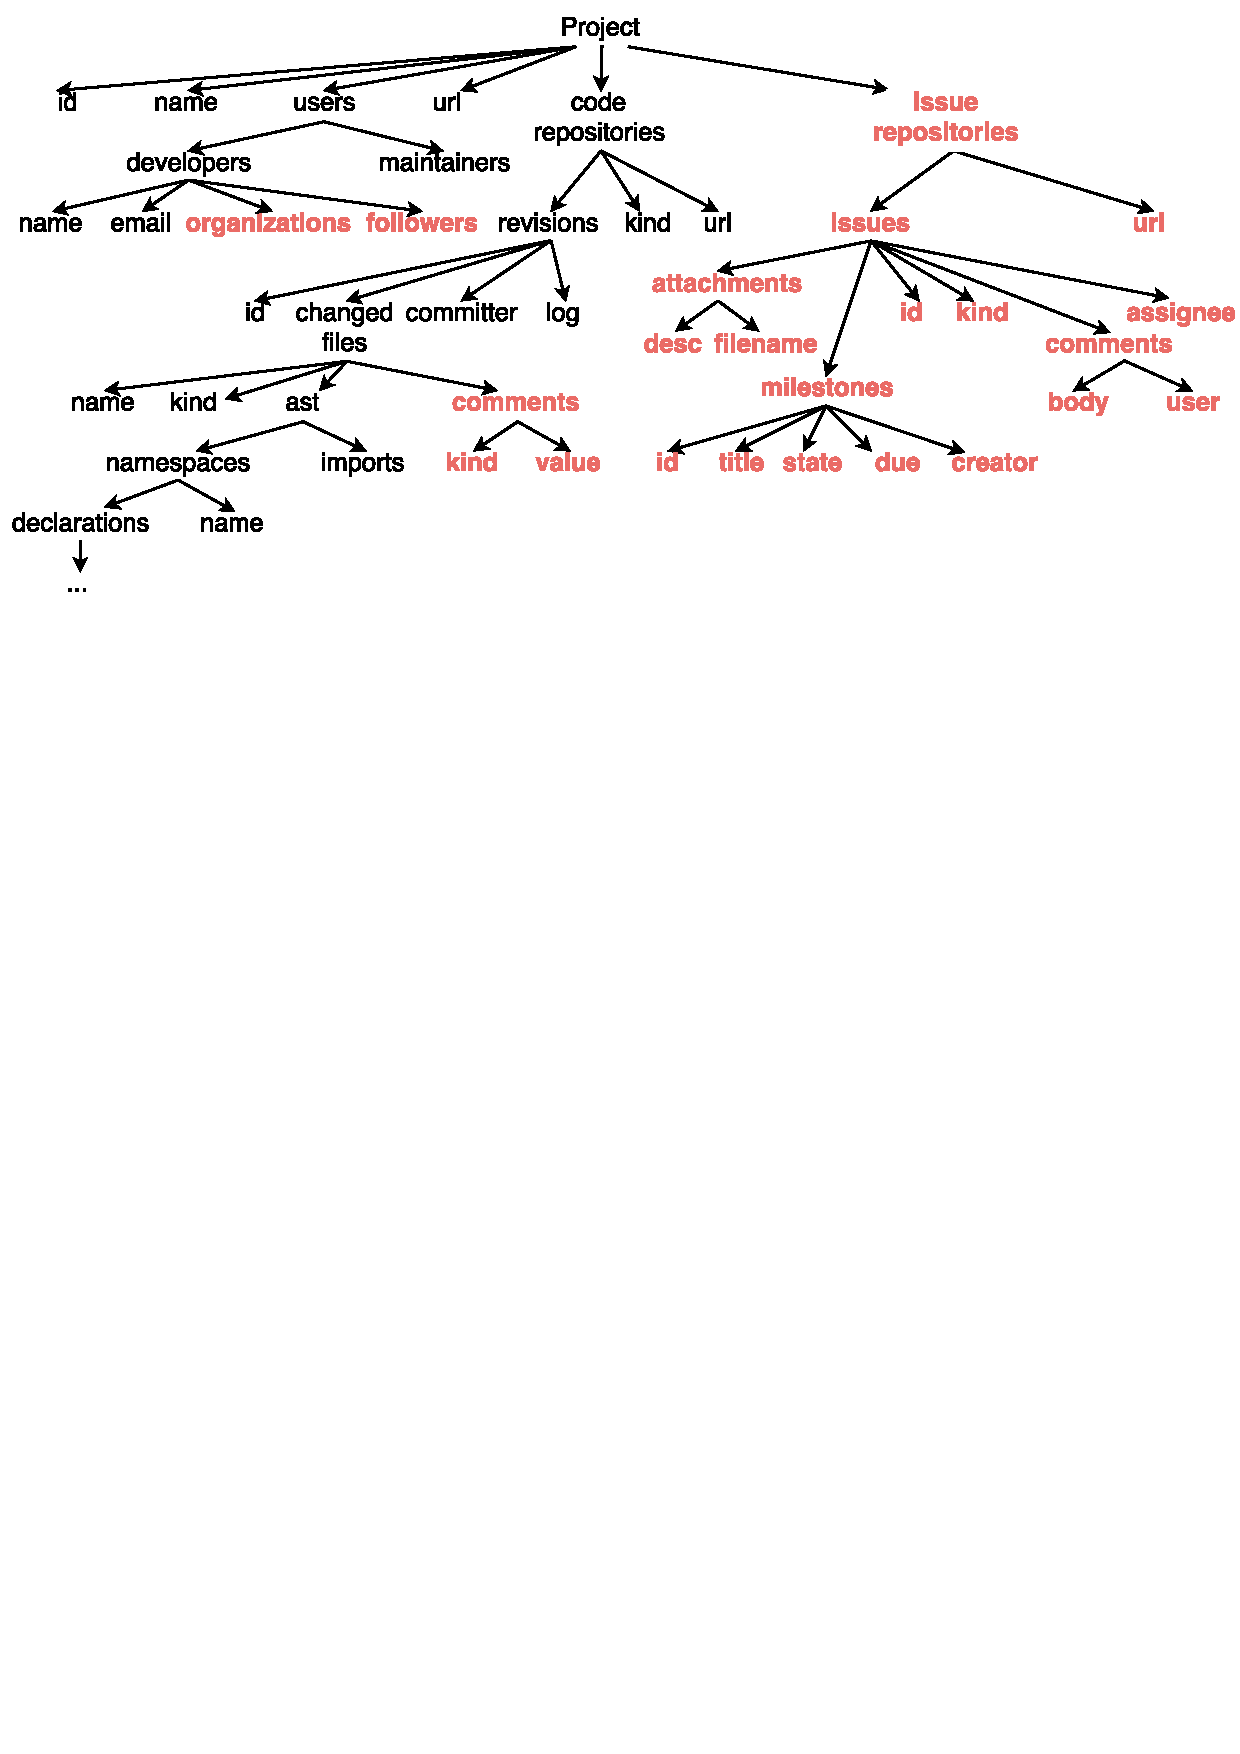
\includegraphics[scale=0.45]{figures/data-schema.pdf}
                    \caption{Candoia's data schema}
                \end{figure}
        \end{frame}

        \begin{frame}
            \frametitle{Few APIs available to Candoia app}
            \begin{itemize}
                \item Running MSR queries (api.boa)
                \item Reading (not writing) files within app (api.fs)
                \item Saving arbitrary data between instances (api.store)
                \item Getting its own package info such as version (api.meta)
                \item Inter-Process-Communication handle (api.ipc)
%                \item Using pre-made views/graphs. (api.view)
            \end{itemize}
            \centering
                \emph{var data = api.boa.run('myprog.boa')}
         \end{frame}

        \begin{frame}
            \frametitle{Candoia Exchange}
            \begin{itemize}
                \item A web platform for sharing MSR apps
                \item Candoia frameworks can connect to exchange for gathering information and  installing apps
            \end{itemize}
         \end{frame}

    \subsection{Platforms}
        \begin{frame}
            \begin{columns}
                \column{0.55\textwidth}
                    \textbf{Moose}
                    \begin{itemize}
                      \item A platforms for reusing of data mining tools.
                      \item Provides scripting and visualizations
                      \item Difference lies in the focus of the tools
                      \item Candoia is focused towards MSR and integrates MSR tools
                    \end{itemize}

                \column{0.55\textwidth}
                \textbf{RepoGrams}
                    \begin{itemize}
                      \item Helps researchers gather evaluation targets and calculate metrices on the target project
                    \end{itemize}
            \end{columns}
        \end{frame}

        \begin{frame}
            \begin{columns}
                \column{0.55\textwidth}
                    \textbf{Kenyon and Sourcerer}
                    \begin{itemize}
                      \item Defines a databse schema for metadata and source code
                      \item Provide access to the dataset via SQL
                    \end{itemize}

                \column{0.55\textwidth}
                    \textbf{Alitheia Core}
                    \begin{itemize}
                      \item Provide a highly extensible framework for analyzing software product
                      \item Process metrics on a large database of open source projects source
                    \end{itemize}
            \end{columns}
         \end{frame}

        \begin{frame}
            \begin{columns}
                \column{0.55\textwidth}
                    \textbf{FLOSSMole}
                    \begin{itemize}
                      \item Analysis on the project metadata
                    \end{itemize}

                \column{0.55\textwidth}
                    \textbf{Groundhog}
                    \begin{itemize}
                      \item Infrastructure for downloading and analysing projects from SourceForge
                    \end{itemize}
            \end{columns}
        \end{frame}


    \subsection{Dataset}
        \begin{frame}
        \textbf{GHTorrent, PROMISE Repository, SourcererDB and Boa}
           \begin{itemize}
                \item Provides standard dataset for evaluation
                \item SourceDB also provides means to create custom dataset
            \end{itemize}
            Focus is on lifting the burden of data curation from user
        \end{frame}

    \subsection{Future Work}
        \begin{frame}
            \frametitle{Future Work}
            \begin{itemize}
                \item Adding new software tools and technologies
                \item Building addiotional useful tools
                \item Utilizing underlying GPUs for better performance
            \end{itemize}
        \end{frame}